%%%%%%%%%%%%%%%%%%%%%%%%%%%%%%%%%%%%%%%%%%%%%%%%%%%%%%%%%%%%%%%%%%%%%%%%%%%%
%% Author template for Management Science (mnsc) for articles with no e-companion (EC)
%% Mirko Janc, Ph.D., INFORMS, mirko.janc@informs.org
%% ver. 0.95, December 2010
%%%%%%%%%%%%%%%%%%%%%%%%%%%%%%%%%%%%%%%%%%%%%%%%%%%%%%%%%%%%%%%%%%%%%%%%%%%%
\documentclass[mnsc,blindrev]{informs3}
%\documentclass[mnsc,nonblindrev]{informs3} % current default for manuscript submission

\OneAndAHalfSpacedXI
%%\OneAndAHalfSpacedXII % Current default line spacing
%%\DoubleSpacedXII
%%\DoubleSpacedXI

% If hyperref is used, dvi-to-ps driver of choice must be declared as
%   an additional option to the \documentclass. For example
%\documentclass[dvips,mnsc]{informs3}      % if dvips is used
%\documentclass[dvipsone,mnsc]{informs3}   % if dvipsone is used, etc.

% Private macros here (check that there is no clash with the style)

%https://tex.stackexchange.com/questions/400692/different-height-of-tikz-subfigures-despite-same-axis-width-height

\usepackage{booktabs}
\usepackage{tabularx}
\usepackage{colortbl}
\usepackage{array}
\usepackage{multirow,calc,amsmath}
\newlength\mylenA
\newlength\mylenB
\newlength\mylenC
\newlength\mylenD
\usepackage{tikz}
\usepackage{tcolorbox}
\usepackage{etoolbox}
\usepackage{algorithm}
\usepackage{algpseudocode}
\usepackage{amsmath}
\usepackage{booktabs}
\AtBeginEnvironment{tcolorbox}{\normalsize}

\usepackage{adjustbox}[valign=t]

\tcbuselibrary{skins, breakable}

\makeatletter
\tcbset{
  tabular/.style={
    boxsep=\z@,top=\z@,bottom=\z@,leftupper=\z@,rightupper=\z@,
    toptitle=1mm,bottomtitle=1mm,boxrule=0.5mm,
    fontupper=\small,
    before upper={\arrayrulecolor{tcbcolframe}\def\arraystretch{1.1}%
      \tcb@hack@currenvir\tabular{#1}},
    after upper=\endtabular\arrayrulecolor{black}},
}
\makeatother

\usepackage{color, colortbl}
\usepackage{graphicx}
%\usepackage{subfigure}
\usepackage{caption}
\usepackage{subcaption}
%\usepackage{tcolorbox}
\usepackage{booktabs}

\usepackage{amsmath}
\usepackage{amsthm}
\usepackage{dsfont}
\usepackage{statmath}
\usepackage{mathtools}
\usepackage{physics}

\usepackage{hyperref}
\usepackage{makecell}
\usepackage{tikz}
\usepackage{pgfplots}
\usepackage{tikzviolinplots}
\usepgfplotslibrary{external}
\tikzexternalize
\usepackage{minted}
\usemintedstyle{gruvbox-light}
\usepackage{scontents}


 
\newcommand{\bx}{\mathbf{x}}
\newcommand{\mD}{\mathcal{D}}
\newcommand{\mG}{\mathcal{G}}
\newcommand{\mM}{\mathcal{M}}
\newcommand{\mE}{\mathcal{E}}
\newcommand{\gray}{\rowcolor[gray]{.90}}
% Natbib setup for author-year style
\usepackage{natbib}
 \bibpunct[, ]{(}{)}{,}{a}{}{,}%
 \def\bibfont{\small}%
 \def\bibsep{\smallskipamount}%
 \def\bibhang{24pt}%
 \def\newblock{\ }%
 \def\BIBand{and}%
\def\pipeline{Explanation Pipeline}
\newcommand{\tw}[1]{\textcolor{red}{Tong: #1}}

\def\checkmark{\tikz\fill[scale=0.4](0,.35) -- (.25,0) -- (1,.7) -- (.25,.15) -- cycle;} 

% \newtheorem{theorem}{Theorem}
% \newtheorem{corollary}{Corollary}[theorem]
% \newtheorem{lemma}[theorem]{Lemma}
% \newtheorem{remark}{Remark}
% \newtheorem{proof}{Proof}


%% Setup of theorem styles. Outcomment only one.
%% Preferred default is the first option.
\TheoremsNumberedThrough     % Preferred (Theorem 1, Lemma 1, Theorem 2)
%\TheoremsNumberedByChapter  % (Theorem 1.1, Lema 1.1, Theorem 1.2)
\ECRepeatTheorems

%% Setup of the equation numbering system. Outcomment only one.
%% Preferred default is the first option.
\EquationsNumberedThrough    % Default: (1), (2), ...
%\EquationsNumberedBySection % (1.1), (1.2), ...

% For new submissions, leave this number blank.
% For revisions, input the manuscript number assigned by the on-line
% system along with a suffix ".Rx" where x is the revision number.
\MANUSCRIPTNO{MS-0001-1922.65}

%%%%%%%%%%%%%%%%
\begin{document}
%%%%%%%%%%%%%%%%

% Outcomment only when entries are known. Otherwise leave as is and
%   default values will be used.
%\setcounter{page}{1}
%\VOLUME{00}%
%\NO{0}%
%\MONTH{Xxxxx}% (month or a similar seasonal id)
%\YEAR{0000}% e.g., 2005
%\FIRSTPAGE{000}%
%\LASTPAGE{000}%
%\SHORTYEAR{00}% shortened year (two-digit)
%\ISSUE{0000} %
%\LONGFIRSTPAGE{0001} %
%\DOI{10.1287/xxxx.0000.0000}%

% Author's names for the running heads
% Sample depending on the number of authors;
% \RUNAUTHOR{Jones}
% \RUNAUTHOR{Jones and Wilson}
% \RUNAUTHOR{Jones, Miller, and Wilson}
% \RUNAUTHOR{Jones et al.} % for four or more authors
% Enter authors following the given pattern:
%\RUNAUTHOR{}

% Title or shortened title suitable for running heads. Sample:
% \RUNTITLE{Bundling Information Goods of Decreasing Value}
% Enter the (shortened) title:
\RUNTITLE{The Illusion of Interpretation}

% Full title. Sample:
% \TITLE{Bundling Information Goods of Decreasing Value}
% Enter the full title:
%change title!!!
\TITLE{Appendix: The Illusion of Interpretation: Post Hoc Explanations Aren't a Silver Bullet for Business Research}

% Block of authors and their affiliations starts here:
% NOTE: Authors with same affiliation, if the order of authors allows,
%   should be entered in ONE field, separated by a comma.
%   \EMAIL field can be repeated if more than one author
\ARTICLEAUTHORS{%
\AUTHOR{Snidely Slippery}
\AFF{Department of Bread Spread Engineering, Dairy University, Cowtown, IL 60208, \EMAIL{slippery@dairy.edu}} %, \URL{}}
\AUTHOR{Marg Arinella}
\AFF{Institute for Food Adulteration, University of Food Plains, Food Plains, MN 55599, \EMAIL{m.arinella@adult.ufp.edu}}
% Enter all authors
} % end of the block

% palette for colorblindness https://davidmathlogic.com/colorblind/#%23000000-%23E69F00-%2356B4E9-%23009E73-%23F0E442-%230072B2-%23D55E00-%23CC79A7

% Sample
%\KEYWORDS{deterministic inventory theory; infinite linear programming duality;
%  existence of optimal policies; semi-Markov decision process; cyclic schedule}

% Fill in data. If unknown, outcomment the field
\KEYWORDS{post hoc, explainable, interpretable} %\HISTORY{This paper was first submitted on April 12, 1922 and has been with the authors for 83 years for 65 revisions.}

\maketitle
preprints
% scopus finds over 400 but doesn't index preprints
%% preprint not necessary
% need to ensure that the papers are actually explaining a black box
% e.g. add
\section{Appendix}
    \subsection{Literature Review}
        \begin{table}[]
        \centering
        \begin{tabular}{l|c}
        \toprule
        \textbf{Web of Science Category}         & \textbf{Number of Papers} \\ \hline
        Operations Research / Management Science & 159                     \\ \hline
        Management                               & 55                      \\ \hline
        Economics                                & 47                      \\ \hline
        Business Finance                         & 42                      \\ \hline
        Business                                 & 31              \\ \bottomrule
        \end{tabular}
        \caption{Number of papers citing either LIME or SHAP that belong to business-adjacent Web of Science categories.}
        \label{tab:citation_count}
    \end{table}

        Table \ref{tab:citation_count} was constructed by using Web of Science to search for publications citing at least one of LIME~\citep{ribeiro16lime} or SHAP~\citep{lundberg17shap} and have either ``LIME" or ``SHAP" appear in the body of the paper.  The results were filtered by the following Web of Science topics: transportation, management, economics, supply chain \& logistics, economic theory, and operations research \& management science. Marketing does not appear in the table because Web of Science does not include it as a distinct category among business adjacent fields.%index any such papers that cited WachterCF~\citep{wachter17wachtercf} or DiCE~\citep{mothilal20dice}.
 
    

%         % allow tuning of DiCE sparsity_weight
%     \subsection{Recourse via Counterfactual Explainer}
%             \label{sec:cf_recourse}
%             A dedicated counterfactual explainer such as DiCE should be used over LIME and SHAP for counterfactual generation. We will show that even when LIME and SHAP are successful in creating counterfactuals $x'$ from a point $x$, their counterfactuals are often more different than $x$ than the ones from DiCE to motivate this claim. To motivate the utility of close counterfactuals using our loan approval example, consider that denied applicants will of course want to make \emph{minimal} changes to their behavior in their quests to be approved in their next applications. 
% %\tw{Feng Lu experiment \# 4: generate DiCE counterfactuals for 1000 data points for model M, and report the percentage of success that the counterfactuals get a different label from G}

%             \paragraph{Success Rate}
%                 To test DiCE's ability to generate true counterfactuals, we generated multiple sets of counterfactuals for the same denied applicants and controlled that the number of features allowed to change in generating each set of counterfactuals was not the same. Specifically, in the context of our data, we defined six features that can be changed, which are: Credit history, income, usage, debt, inquiries, credit score, while features such as age, sex, and married were considered immutable features. %Moreover, we specify that those features that can be changed can only be changed within a small range (within one standard deviation), which is set both to be consistent with the setting in Section 4.2.1 and to make the experiment more realistic, since the range in which denied applicants can change their features is always limited. 
%                 We define the success rate of generating counterfactuals for each applicant as follows. For example, when an applicant is allowed to change $K$ features to generate counterfactuals, they have a total of $C_{6}^{k}$ ways to generate counterfactuals, and the ratio of the number of successful counterfactuals generated in these ways to $C_{6}^{k}$ is the success rate of generating counterfactuals for the applicant.

%                 % THIS CONFLICTS WITH HIGH SUCCESS RAT EFROM LIME/SHAP
%                 As Figure 8 shows, although increasing the number of features that can be changed can significantly increase the percentage of applicants accepted. But even then, the highest success rate is only about 12\%. This suggests that even using a popular counterfactual generation algorithm like DiCE may have difficulty informing actionable recourse. With such a low success rate, applicants would often be wasting their time with recourse recommended by DiCE. 

            
%             \begin{figure}[ht!]
%                 \centering
%                 \includegraphics[width=0.8\textwidth]{old_files/Figures/feng_fig/sparsity_dice.png}
%                 \caption{Percentages of times DiCE was able to produce true counterfactuals for rejected applicants for different sparsity parameters.}
%                 \label{fig:dice_sparsity}
%             \end{figure}

%\subsection{Justification for Metrics}

    
    \subsection{Details and Additional Experiments for Section 5.1}
            \begin{table}[]
            % determine target width of combined cols 2 and 3:
            \settowidth\mylenA{Correlated \\ Features} 
            % determine usable width of cols 2 and 3:
            \setlength\mylenB{(\mylenA-3\tabcolsep)/3}
            \centering
            \begin{tabular}{|c|*{3}{wc{\mylenB}|}*{3}{wc{\mylenB}|}*{3}{wc{\mylenB}|}}
            \hline
            \textbf{Experiment} & \multicolumn{3}{c|}{\makecell{\textbf{Correlated} \\ \textbf{Features}}} & \multicolumn{3}{c|}{\makecell{\textbf{Unobserved} \\ \textbf{Confounder}}} & \multicolumn{3}{c|}{\makecell{\textbf{Observed} \\  \textbf{Confounder}}} \\ \hline
            \textbf{Feature} & \textbf{$\mathcal{G^*}$} & \textbf{$\mathcal{G_{\text{effect}}}$} & \textbf{$\mathcal{M}$}             
            &   \textbf{$\mathcal{G}^*$} & \textbf{$\mathcal{G_{\text{effect}}}$} & \textbf{$\mathcal{M}$}              & \textbf{$\mathcal{G}^*$} & \textbf{$\mathcal{G_{\text{effect}}}$}             & \textbf{$\mathcal{M}$}             \\ \hline
            Age              & \checkmark& \textcolor{red}{\checkmark}    & \checkmark                                                            & \checkmark  & \checkmark    & \checkmark                               & \checkmark& \checkmark   & \checkmark                               \\ \hline
            Sex              & \checkmark& \checkmark & \checkmark   & \checkmark  & \checkmark   & \checkmark                                & \checkmark& \checkmark & \checkmark                                 \\ \hline
            Inquiries        & \checkmark& \checkmark  & \checkmark &  \checkmark     &\multicolumn{1}{c|}{\checkmark}        & \checkmark & \checkmark & \textcolor{red}{\checkmark}    & \checkmark                     \\ \hline
            Cosigner         & \checkmark& \checkmark   & \checkmark                                                              & \checkmark  & \checkmark                                   & \checkmark& \checkmark & \checkmark  &\multicolumn{1}{c|}{\checkmark}                                \\ \hline
            Utilization      & \checkmark& \checkmark  & \checkmark                                                                 & \checkmark  & \checkmark   & \checkmark                                & \checkmark& \textcolor{red}{\checkmark}  & \checkmark                                \\ \hline
            Credit Score     & \checkmark& \textcolor{red}{\checkmark} & \checkmark                                 &                               & \checkmark  & \checkmark  & \checkmark & \textcolor{red}{\checkmark}  & \checkmark                                \\ \hline
            %Credit Score 2   & \multicolumn{1}{c|}{}    &\multicolumn{1}{c|}{}                               &                                    & \multicolumn{1}{c|}{}                                & \textcolor{red}{\checkmark}                                 & \multicolumn{1}{c|}{\checkmark}  & \multicolumn{1}{c|}{}                                    &                                     & \multicolumn{1}{c|}{}   & \multicolumn{1}{c|}{}                                 &      &\multicolumn{1}{c|}{}                               \\ \hline
            Social Support   & \multicolumn{1}{c|}{}    & \multicolumn{1}{c|}{}                               &                                    &  \multicolumn{1}{c|}{}  & \multicolumn{1}{c|}{\textcolor{red}{\checkmark}} & \multicolumn{1}{c|}{} & \multicolumn{1}{c|}{}                                 &\multicolumn{1}{c|}{}             &\multicolumn{1}{c|}{}                      \\ \hline
            Income & \multicolumn{1}{c|}{}    & \multicolumn{1}{c|}{}      &     & \multicolumn{1}{c|}{}                                       & \multicolumn{1}{c|}{\textcolor{red}{\checkmark}} & \multicolumn{1}{c|}{} & \multicolumn{1}{c|}{}                                  &\multicolumn{1}{c|}{}  &\multicolumn{1}{c|}{}                                 \\ \hline
            \end{tabular}
            \caption{Table indicating whether the ground truth models $\mathcal{G}^*$ and $\mathcal{G}_{\text{effect}}$ use each feature  and whether $\mathcal{M}$ has access to each feature in data produced by ground truth models using them in each experiment. Features which are correlated in $\mathcal{G}_{\text{effect}}$ in order to violate causal inference conditions are marked red.} 
            \label{tab:simulated_variations}
            \end{table}
            
        \subsubsection{Correlated Features}
            To isolate the individual data-related effects in each experiment, we will create an ideal data generator $\mathcal{G}^*$ together with a data generator $\mathcal{G}_{\text{effect}}$ symptomatic of each effect. $\mathcal{G}^*$ generates data that satisfies causal inference conditions. That is, all features are pairwise independent, observed, and unconfounded.
        
            We then compare the abilities of LIME and SHAP to explain models $\mathcal{M}$ trained on data generated by $\mathcal{G}^*$ and $\mathcal{G}_{\text{effect}}$ for each effect. Following the experimental setup of Section \ref{sec:unfaithfulness}, each experiment will be represented by a plot of the metric of interest for that experiment computed using LIME and SHAP explanations of models $\mathcal{M}$ trained on 100 applicants from the test sets of data given by both $\mathcal{G}^*$ and $\mathcal{G}_{\text{effect}}$.  At the end of this section, we also investigate the desirable situation where LIME and SHAP explain an MLP model $\mathcal{M}$ with reasonable accuracy trained on the data from $\mathcal{G}^*$ to demonstrate that explanations of $\mathcal{M}$ are still imperfect even if the data satisfies causal inference conditions. 
    
            In this section, the model data generators $\mathcal{G}^*$ use a simplified set of features. Namely, age, sex, credit inquiries, credit utilization, credit score, and availability of a cosigner. All features are independent of each other. When training the models $\mathcal{M}$ on $\mathcal{G}^*$ and $\mathcal{G}_{\text{effect}}$, we have the setup where 5000 applicants are generated and $\mathcal{M}$ is an MLP with ROC AUC at least .85. Table \ref{tab:simulated_variations} illustrates which features are used as inputs to each ground truth model $\mathcal{G}^*$ and $\mathcal{G}_{\text{effect}}$, as well as which features are involved in the effect in $\mathcal{G}_{\text{effect}}$ that breaks the causal inference conditions. It also marks when $\mathcal{M}$ has access to a feature in training data provided by ground truth model using that feature. %For each experiment, $\mathcal{M}$ has 3-5 hidden layers and is trained for sufficiently many iterations so that its ROC AUC is between 80\% and 85\%. 
        
            %With enough observations, you will eventually be able to identify the separate effects of even highly collinear (but never perfectly collinear) variables. This is why Rob Franzese and UMich likes to call multicollinearity "micronumerosity."
        
            Figure \ref{fig:lime_shap_colinear_ranks} shows bar plots of the rankings for the age and credit score feature by LIME and SHAP before and after making age and credit score strongly correlated. The bar plots show that the dependency between age and credit score is associated with a decrease of age's rank and an increase of credit score's rank for both LIME and SHAP. This is because when credit score depends on age, it becomes a more powerful predictor of loan approval that is more useful to $\mathcal{M}$ than age. This is a concrete illustration of how explainers allocate the most importance to features which are the most useful predictors of the target for the black box. 
            \begin{figure}[ht!]
                \centering
                \begin{subfigure}{.27\textwidth}
                  \centering
                  \captionsetup{justification=centering}
                  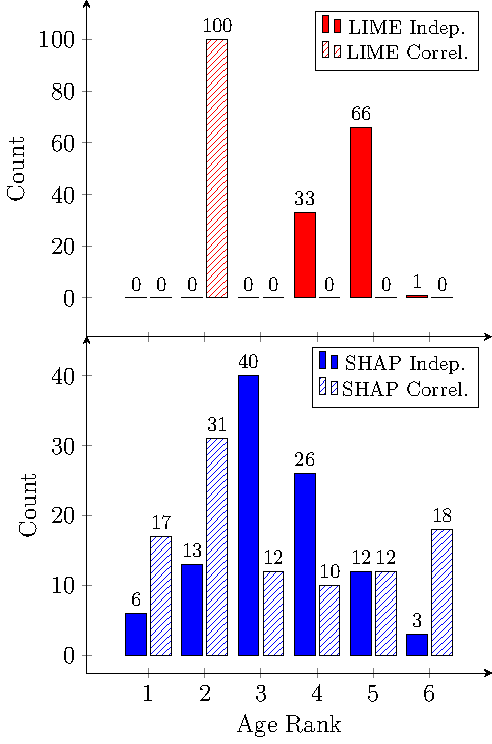
\includegraphics[width=\textwidth]{FinalFigures/sec4_3_corr_ranks_age_final.pdf}%{Figures/fig_age_col.pdf}%{Figures/lime_spearman_colinear.png}
                                %\includegraphics[width=.9\linewidth]{Figures/lime_shap_Spearman_magnitude.png}
    
                  \caption{Age}%Spearman rank correlations of ranked feature importance magnitudes from LIME against the true ranked magnitudes from $\mathcal{G}$.}
                   \label{fig:age_colinear}
                \end{subfigure}%
                \hspace{3cm}
                \begin{subfigure}{.27\textwidth}
                  \centering
                     \captionsetup{justification=centering}
                  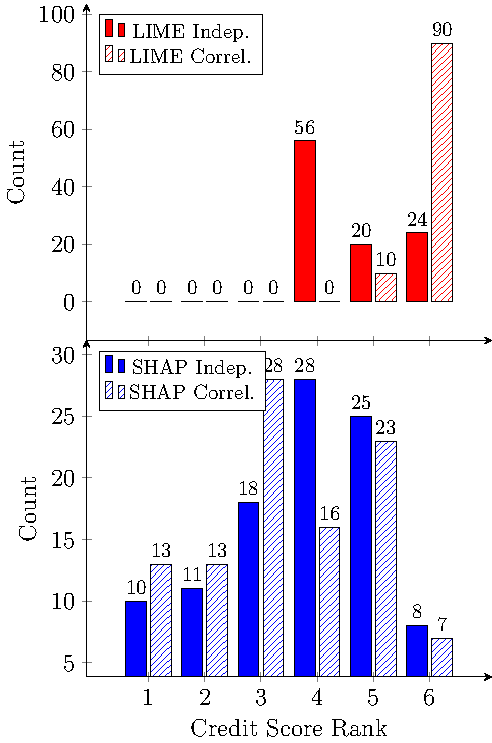
\includegraphics[width=\textwidth]{FinalFigures/sec4_3_corr_ranks_score_final.pdf}%{Figures/fig_score_col.pdf}%{Figures/shap_spearman_colinear.png}
    
                  %\includegraphics[width=.9\linewidth]{Final_Figures/fig9b.png}%{Figures/shap_spearman_colinear.png}
                  \caption{Credit Score}%Spearman rank correlations of signed feature importance magnitudes from LIME and SHAP against the true ranking from $\mathcal{G}$.}
                   \label{fig:score_colinear}
                \end{subfigure}
                
                \caption{Bar charts showing how LIME and SHAP incorrectly identify credit score as being important because it being a statistical summary of other features makes it a good predictor, and hence important to the $\mathcal{M}$ but not $\mathcal{G}$.}%rankings of age and credit score change from when being independent to when credit score becomes a function of age}
                \label{fig:lime_shap_colinear_ranks}
            \end{figure}

        \subsubsection{Observed Confounding}
            \label{sec:appendix_obs_conf}
            An observed confounding problem can cause an unimportant but confounded feature to be identified as important. Observed confounding is a special case of correlation with the additional conditions that the correlation is actually causal and that one of the features has a causal impact on both the other feature and the target variable. Whereas the experiment involving correlated features showed that credit score becoming a function of age caused age to lose importance, we will show how credit score can be set to be irrelevant to loan approval, but nevertheless be given undue importance when it has an observed confounding problem. The reason for this is again because the ML model views credit score as an exceptional predictor, but this exposition is still worthwhile because the resulting effect is distinct from that of mere correlation.  
    
            To demonstrate this problem, we construct $\mathcal{G}_{\text{confounded}}$ with two important changes. First, the credit score becomes a function of credit utilization and credit inquiries. Second, credit score is not a direct cause of loan approval but nevertheless appears in the dataset. A problem arises because the credit score feature contains redundant information about credit utilization and credit inquiries. This experimental setup is different from our experiment that demonstrates the problematic nature of correlation because in that experiment both of the correlated features had a causal impact on loan approval. In this experiment credit score does not have a causal impact on loan approval.

              \begin{figure}[ht!]
                \centering
                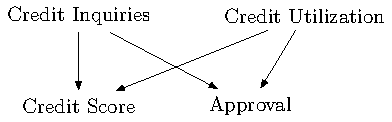
\includegraphics[width=.27\textwidth]{AppendixFigures/dags-figure1.pdf}
                
                \caption{Causal graph explaining the relationships of credit utilization, credit inquiries, and credit score for the experiment involving observed confounding}
                \label{fig:unobs_conf_dag}
            \end{figure}

        
            Our experiment explaining an MLP trained on $\mathcal{G}_{\text{confounded}}$ demonstrates that unimportant confounded features can nevertheless be identified as important by LIME and SHAP. The violin plots for the distributions of the importance of the credit score feature in Figure \ref{fig:lime_score} show that, for LIME, credit score importance is larger when confounded than otherwise, even though the confounded credit score is unimportant. SHAP does not exhibit exactly the same behavior, but Figure \ref{fig:shap_score} does show that when credit score is confounded, its importance distribution has more mass above 0 than otherwise. This type of scenario is problematic in practice because although researchers can easily tell if a set of features are correlated, it is much more difficult to know how the features causally impact each other and the outcome of interest. 


    
            \begin{figure}[ht!]
                \centering
                \begin{subfigure}{.27\textwidth}
                  \centering
                  \captionsetup{justification=centering}
                  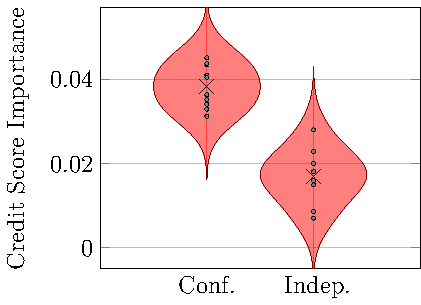
\includegraphics[width=\textwidth]{Figures/sec4_3_obsconf_lime.pdf}%{Figures/fig_obs_conf_score_ranks_a.pdf}%{Final_Figures/fig11a.png}%{Figures/lime_cosigner.png}
                  \caption{LIME}
                   \label{fig:lime_score}
                \end{subfigure}%
                \hspace{3cm}
                \begin{subfigure}{.27\textwidth}
                  \centering
                   \captionsetup{justification=centering}
                  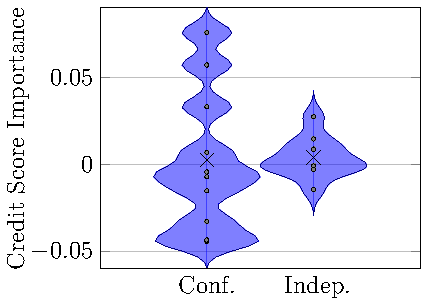
\includegraphics[width=\textwidth]{Figures/sec4_3_obsconf_shap.pdf}%{Figures/fig_obs_conf_score_ranks_b.pdf}%{Final_Figures/fig11b.png}%{Figures/shap_cosigner.png}
                  \caption{SHAP}
                   \label{fig:shap_score}
                \end{subfigure}
                
                \caption{Violin plots of importance values of \emph{credit score} from LIME and SHAP for cases when \emph{credit score} is unconfounded and confounded by the observed credit utilization and credit inquiries features.}
               \label{fig:lime_shap_score}
            \end{figure}
        
        \subsubsection{Unobserved Confounding}
            \label{sec:appendix_unobs_conf}
            To illustrate the effects of unobserved confounders on explanation quality, we design $\mathcal{G}^*$ and $\mathcal{G}_{\text{unobserved confounding}}$ to differ based on the role of the social support feature. $\mathcal{G^*}$ is set such that social support is not a factor at all and $\mathcal{G}_{\text{unobserved confounding}}$ is set to have a measure of social support that confounds income and is not observable by $\mathcal{M}$. In $\mathcal{G}_{\text{unobserved confounding}}$, we set social support to negatively affect income under the supposition that individuals with high social support receive extra money and services such that they have less incentive to have a large income from their employment. Thus, social support is an indirect cause for loan approval. 
            
            $\mathcal{G}^*$ is designed to differ from $\mathcal{G}_{\text{unobserved confounding}}$ in that the social support feature does not exist, and all features are mutually independent. We assume that social support has no importance in both $\mathcal{G}^*$ and $\mathcal{M}$.%$ so that feature rankings are directly comparable between the two.

            \begin{figure}[ht!]
                \centering
                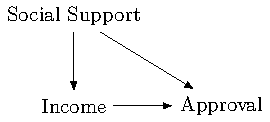
\includegraphics[width=.27\textwidth]{AppendixFigures/dags-figure0.pdf}
                
                \caption{Causal graph explaining the nature of social support for the experiment involving unobserved confounding}
                \label{fig:unobs_conf_dag}
            \end{figure}
            
        
            Paradoxically, explanations of the model trained on confounded data imply that having a high income lowers the chances of getting a loan application approved. This can be seen clearly in the violin plots of the importance of the income feature shown in Figure \ref{fig:lime_income}. The distribution of importance for income is contained in the negative region when income is confounded by social support. The opposite is true for the explanations of the model trained on the data with independent, unconfounded features. Figure \ref{fig:shap_income} shows that for SHAP a lesser effect is present; the left tail of the income importance distribution is heavier than the right tail. This example establishes the possibility for researchers to come away with a completely incorrect understanding of an unobserved confounder's causal descendants. 




            \begin{figure}[ht!]
                \centering
                \begin{subfigure}{.27\textwidth}
                  \centering
                  \captionsetup{justification=centering}
                  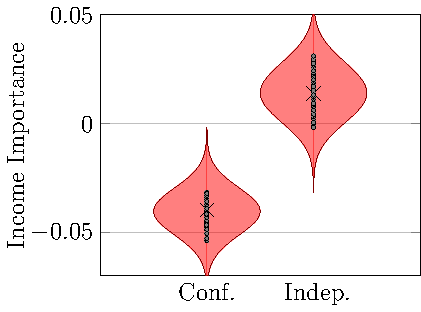
\includegraphics[width=\textwidth]{Figures/sec4_3_conf_lime.pdf}%{Figures/lime_income.pdf}%{Figures/lime_spearman_colinear.png}
                                %\includegraphics[width=.9\linewidth]{Figures/lime_shap_Spearman_magnitude.png}
    
                  \caption{LIME}%Spearman rank correlations of ranked feature importance magnitudes from LIME against the true ranked magnitudes from $\mathcal{G}$.}
                   \label{fig:lime_income}
                \end{subfigure}%
                \hspace{3cm}
                \begin{subfigure}{.27\textwidth}
                  \centering
                     \captionsetup{justification=centering}
                  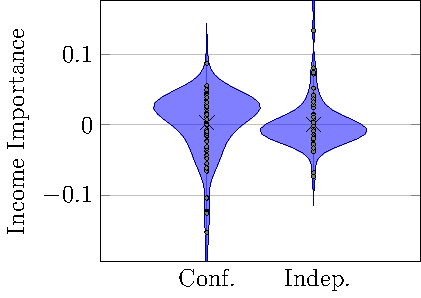
\includegraphics[width=\textwidth]{Figures/sec4_3_conf_shap.pdf}%{Figures/shap_income.pdf}%{Figures/shap_spearman_colinear.png}
    
                  %\includegraphics[width=.9\linewidth]{Final_Figures/fig9b.png}%{Figures/shap_spearman_colinear.png}
                  \caption{SHAP}%Spearman rank correlations of signed feature importance magnitudes from LIME and SHAP against the true ranking from $\mathcal{G}$.}
                   \label{fig:shap_income}
                \end{subfigure}
                
                \caption{Violin plots of feature importance values for \emph{income} from LIME and SHAP for cases when \emph{income} is unconfounded and confounded by the unobserved social support feature}
                \label{fig:lime_shap_income}
            \end{figure}

    \subsection{Details and Additional Experiments Related to Inconsistency}
        \label{sec:appendix_inconsistency}

        \subsubsection{Instability Due to Decision Boundary Volatility}         
            \label{sec:instability}
            Intuitively, explanations for the outcomes occuring in similar scenarios should be similar as well. In fact, the reasoning behind the decisions made on applicants with sufficiently similar profiles should be identical. Otherwise, applicants could have reason to suspect unfairness. But consider a situation where inputs $\xi^{(1)}$ and $\xi^{(2)}$ are nearby but $\mathcal{M}(\xi^{(1)})$ and $\mathcal{M}(\xi^{(2)})$ are distant. If one only cares about the faithfulness of the explainer with respect to $\mathcal{M}$, the explanations of $\xi^{(1)}$ and $\xi^{(2)}$ should definitely be dissimilar. However, if we care about faithfulness with respect to $\mathcal{G}$, and $\mathcal{G}(\xi^{(1)})$ and $\mathcal{G}(\xi^{(2)})$ are close, instability is not desirable. Instability is therefore a problem when an explainer is too unstable due to, e.g., overfitting. Both when $\mathcal{M}$ overfits $\mathcal{G}$ and when $\mathcal{E}$ overfits $\mathcal{M}$ can cause unnecessary variability to be captured by $\mathcal{E}$ and result in unnecessary instability. 
          
            To demonstrate instability, we construct a two-dimensional loan approval model based only on income and credit utilization and check the instability of LIME's coefficients when overfitting is and is not present. %Our approach for evaluating stability is similar to the coefficient stability index (CSI) from \citep{visani21stability}. 
            The first step of the experiment is to generate a dataset using a ground truth model $\mathcal{G}$ which decides approval using a linear combination of income and credit utilization. Then we train an MLP $\mathcal{M}_1$ on a noisy version of that dataset where some points near the decision boundary of $\mathcal{G}$ have their label flipped. $\mathcal{M}_1$ misclassifies those noise points and is therefore meant to represent a classifier that did not overfit by fitting the noise points correctly. We construct another MLP $\mathcal{M}_{2}$ which does overfit the noisy data and consequently has a comparatively erratic decision boundary. The decision boundaries of $\mathcal{M}_1$ and $\mathcal{M}_2$ are shown in Appendix Section \ref{sec:effect_of_overfitting}. Finally, we quantify coefficient stability by computing the Euclidean distances between the LIME coefficients for pairs of LIME explanations of points near the decision boundary of $\mathcal{M}_1$ and their nearest neighbor with the same label. 

            Figure \ref{fig:dbd_dists} shows that explainers for $\mathcal{M}_{2}$ are more unstable than those for $\mathcal{M}_1$. This is evident because the distances between the coefficient sets of LIME explainers for pairs of nearby points are always much higher for LIME explainers of $\mathcal{M}_{2}$ than for explainers of $\mathcal{M}_1$.% When explaining $\mathcal{M}$, the mean distance is $9e-4$ and the standard deviation is $1e-3$, while when explaining $\mathcal{M}_{\text{overfit}}$, the mean distance is $2e-2$ and the standard deviation is $1.7e-2$. Explainers of $\mathcal{M}$ have high coefficient stability because the distances are concentrated near 0 in Figure \ref{fig:dbd_dists}. Explainers of $\mathcal{M}_{\text{overfit}}$ do not because the distance distribution is always much larger than 0. 

            \begin{figure}[ht!]
                \centering
                % \begin{subfigure}[t]{.3\textwidth}
                %   \centering
                %   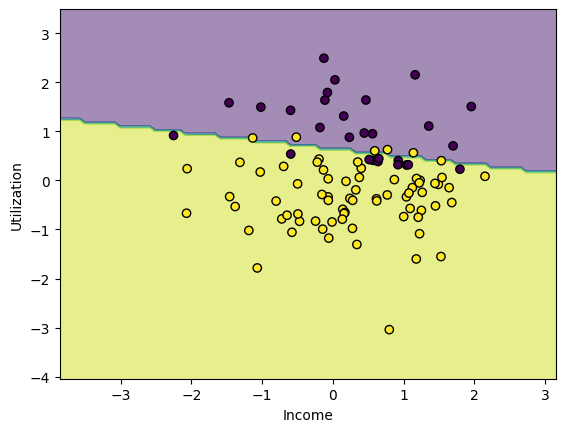
\includegraphics[width=\textwidth]{Figures/dbd_M.png}
                %   \caption{Decision boundary of $\mathcal{M}$}
                %   \label{fig:M_dbd}
                % \end{subfigure}%
                % \hfill
                % \begin{subfigure}[t]{.3\textwidth}
                %   \centering
                %   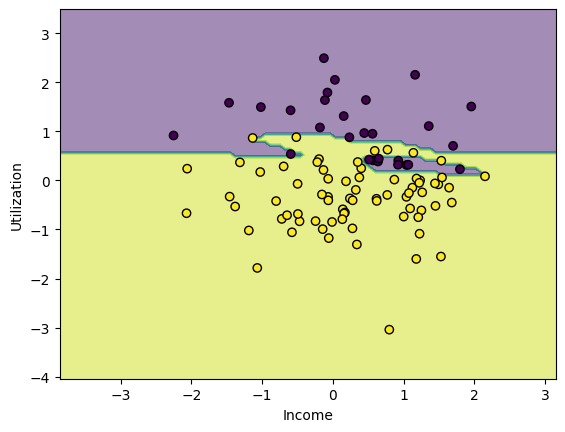
\includegraphics[width=\textwidth]{Figures/dbd_Mp.png}
                %   \caption{Decision Boundary of $\mathcal{M}_{\text{overfit}}$}
                %   \label{fig:Mp_dbd}
                % \end{subfigure}
                % \hfill
               \begin{subfigure}[t]{.27\textwidth}
                \centering
                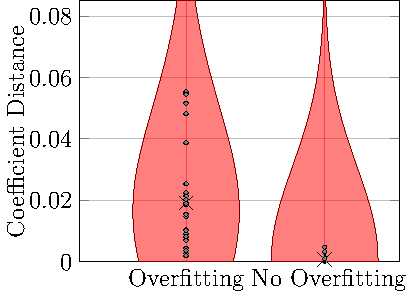
\includegraphics[width=\textwidth]{Figures/sec5_1_overfitting_spearmans.pdf}%{Figures/dbd_dists.png}
                \caption{Effect of overfitting on stability}%Violin plots representing the stability of explainers of $\mathcal{M}$ and $\mathcal{M}_{\text{overfit}}$}
                \label{fig:dbd_dists}
                \end{subfigure}
                \caption{Violin plots representing the stability of explainers of $\mathcal{M}_1$ and $\mathcal{M}_2$. Each point represents the $L_2$ distance between the LIME coefficients for the explanation of a point near the decision boundary of $\mathcal{G}$ and its closest neighbor of the same class.}
                \label{fig:effect_of_overfitting}
            \end{figure}
            

        
            \subsubsection{Decision Boundaries for Section on Decision Boundary Volatility}
                \label{sec:effect_of_overfitting}
                \begin{figure}[ht!]
                    \centering
                    \begin{subfigure}[t]{.27\textwidth}
                      \centering
                      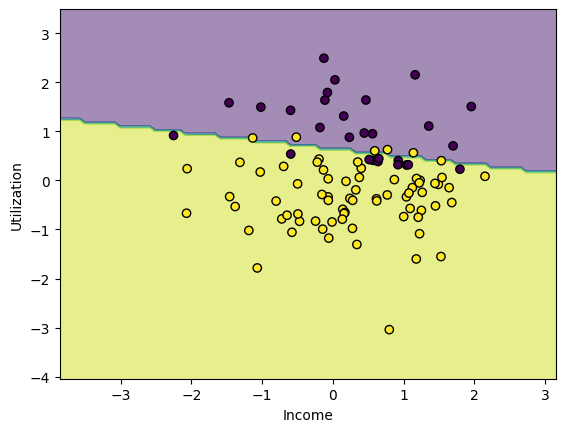
\includegraphics[width=\textwidth]{Figures/dbd_M.png}
                      \caption{Decision boundary of $\mathcal{M}$}
                      \label{fig:M_dbd}
                    \end{subfigure}%
                    \hspace{1cm}
                    \begin{subfigure}[t]{.27\textwidth}
                      \centering
                      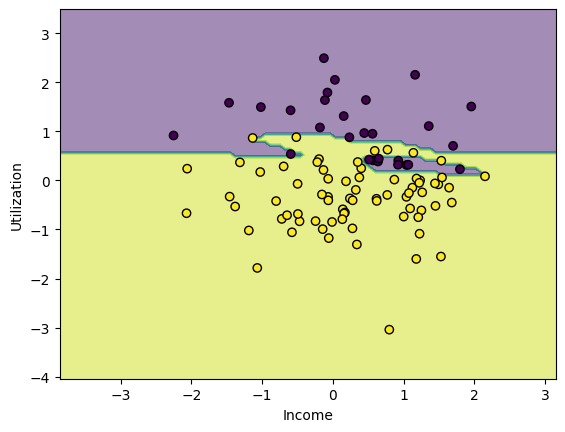
\includegraphics[width=\textwidth]{Figures/dbd_Mp.png}
                      \caption{Decision Boundary of $\mathcal{M}_{\text{overfit}}$}
                      \label{fig:Mp_dbd}
                    \end{subfigure}
                    \hspace{1cm}
                   \begin{subfigure}[t]{.27\textwidth}
                    \centering
                    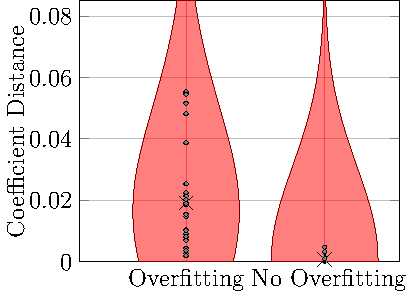
\includegraphics[width=\textwidth]{Figures/sec5_1_overfitting_spearmans.pdf}%{Figures/dbd_dists.png}
                    \caption{Effect of overfitting on stability}%Violin plots representing the stability of explainers of $\mathcal{M}$ and $\mathcal{M}_{\text{overfit}}$}
                    \label{fig:dbd_dists}
                    \end{subfigure}
                    \caption{Visualizations of decision boundaries for MLPs that do and do not overfit ($\mathcal{M}$ and $\mathcal{M}_{\text{overfit}}$) on a simple two variable loan approval dataset. Yellow points are accepted applicants and purple points are denied applicants.}
                    \label{fig:dbds}
                \end{figure}
        
        \subsubsection{Effect of Data Pre-processing}
        We identify two ways data preprocessing can affect post hoc explanations. First, the preprocessing affects the decision boundaries of models trained on it, which we know from Section \ref{sec:} affects explanations. Second, preprocessing routines like standardization can change the signs of feature values, which we know from Section \ref{sec:theoretical_considerations} can cause the Shapley value sign to differ from that of $\beta$. 

    
            \begin{figure}[ht!]
                \centering
                \begin{subfigure}{.27\textwidth}
                  \centering
                  \captionsetup{justification=centering}
                  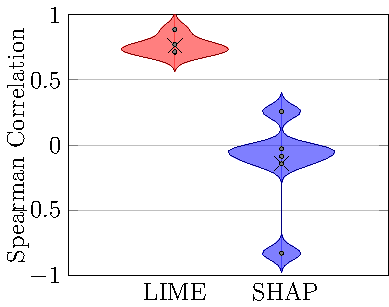
\includegraphics[width=\textwidth]{AppendixFigures/apx_preproc_rank_corrs.pdf}
                  \caption{Correlations between feature rankings from explanation of model trained on standardized data with feature rankings from explanations of model trained on data with no preprocessing}%Spearman rank correlations of ranked feature importance magnitudes from LIME against the true ranked magnitudes from $\mathcal{G}$.}
                   \label{fig:lime_income}
                \end{subfigure}%
                \caption{}%Violin plots of feature importance values for \emph{income} from LIME and SHAP for cases when \emph{income} is unconfounded and confounded by the unobserved social support feature}
                \label{fig:lime_shap_preproc_corr}
            \end{figure}
    
    \subsection{Additional Mitigation Strategies}
        \label{sec:appendix_mitigations}
        \subsubsection{Averaging Explanations across Explainers}
            \label{sec:averaging_across_explainers}
            We previously showed that LIME and SHAP explanations are often uncorrelated, which is problematic since there is no way to know which one is giving a better explanation. We attempt to resolve this issue by aggregating their rankings. We average the rankings instead of the feature importance values because the feature importance values have different meanings. To aggregate a ranking from LIME and a ranking from SHAP we use the Borda count to generate a new ranking. % from LIME and SHAP over their hyperparameters and random seeds. 
            %Specifically, we sample 100 applicants from the data, produce a set of LIME explanations of these applicants by varying the random seed, and produce another set by varying the kernel width. Likewise, for each applicant, we produce sets of SHAP explanations created by varying SHAP's random seed and $nsamples$ parameter. An average explanation is then constructed by averaging the feature importance values from the component explanations and then ranking the features accordingly. Additional methods for aggregating LIME and SHAP are tested in the Appendix. 

            We did not find evidence that averaging LIME and SHAP together is beneficial. Figure \ref{fig:lime_shap_Spearman_together} shows that the averaged explanations were usually worse than those from LIME. We propose that this is because LIME and SHAP explanations generally do not satisfy criteria necessary for ensemble learning to be successful. %The distribution of Spearman correlations for averaged explanations has both a lower median and larger variance than the distribution for LIME. The opposite is true for SHAP; the averaged explanations have a higher median correlation and lower variance. But, comparing the distributions for LIME, SHAP, and LIME+SHAP, it is clear that just using LIME alone is the best option, at least in this experiment. The effect of averaging LIME and SHAP together on recall is subtle; the median recall for LIME+SHAP is marginally higher than the recalls for LIME and SHAP individually.  

            %use fbox to tailor crop
            \begin{figure}[ht!]
            \centering
                \begin{subfigure}{.27\textwidth}
                \centering
                %\fbox{\includegraphics[width=\textwidth,trim=0 10 70 70 mm, clip=true]{Figures/fig21.pdf}}%{Final_Figures/fig20.png}
                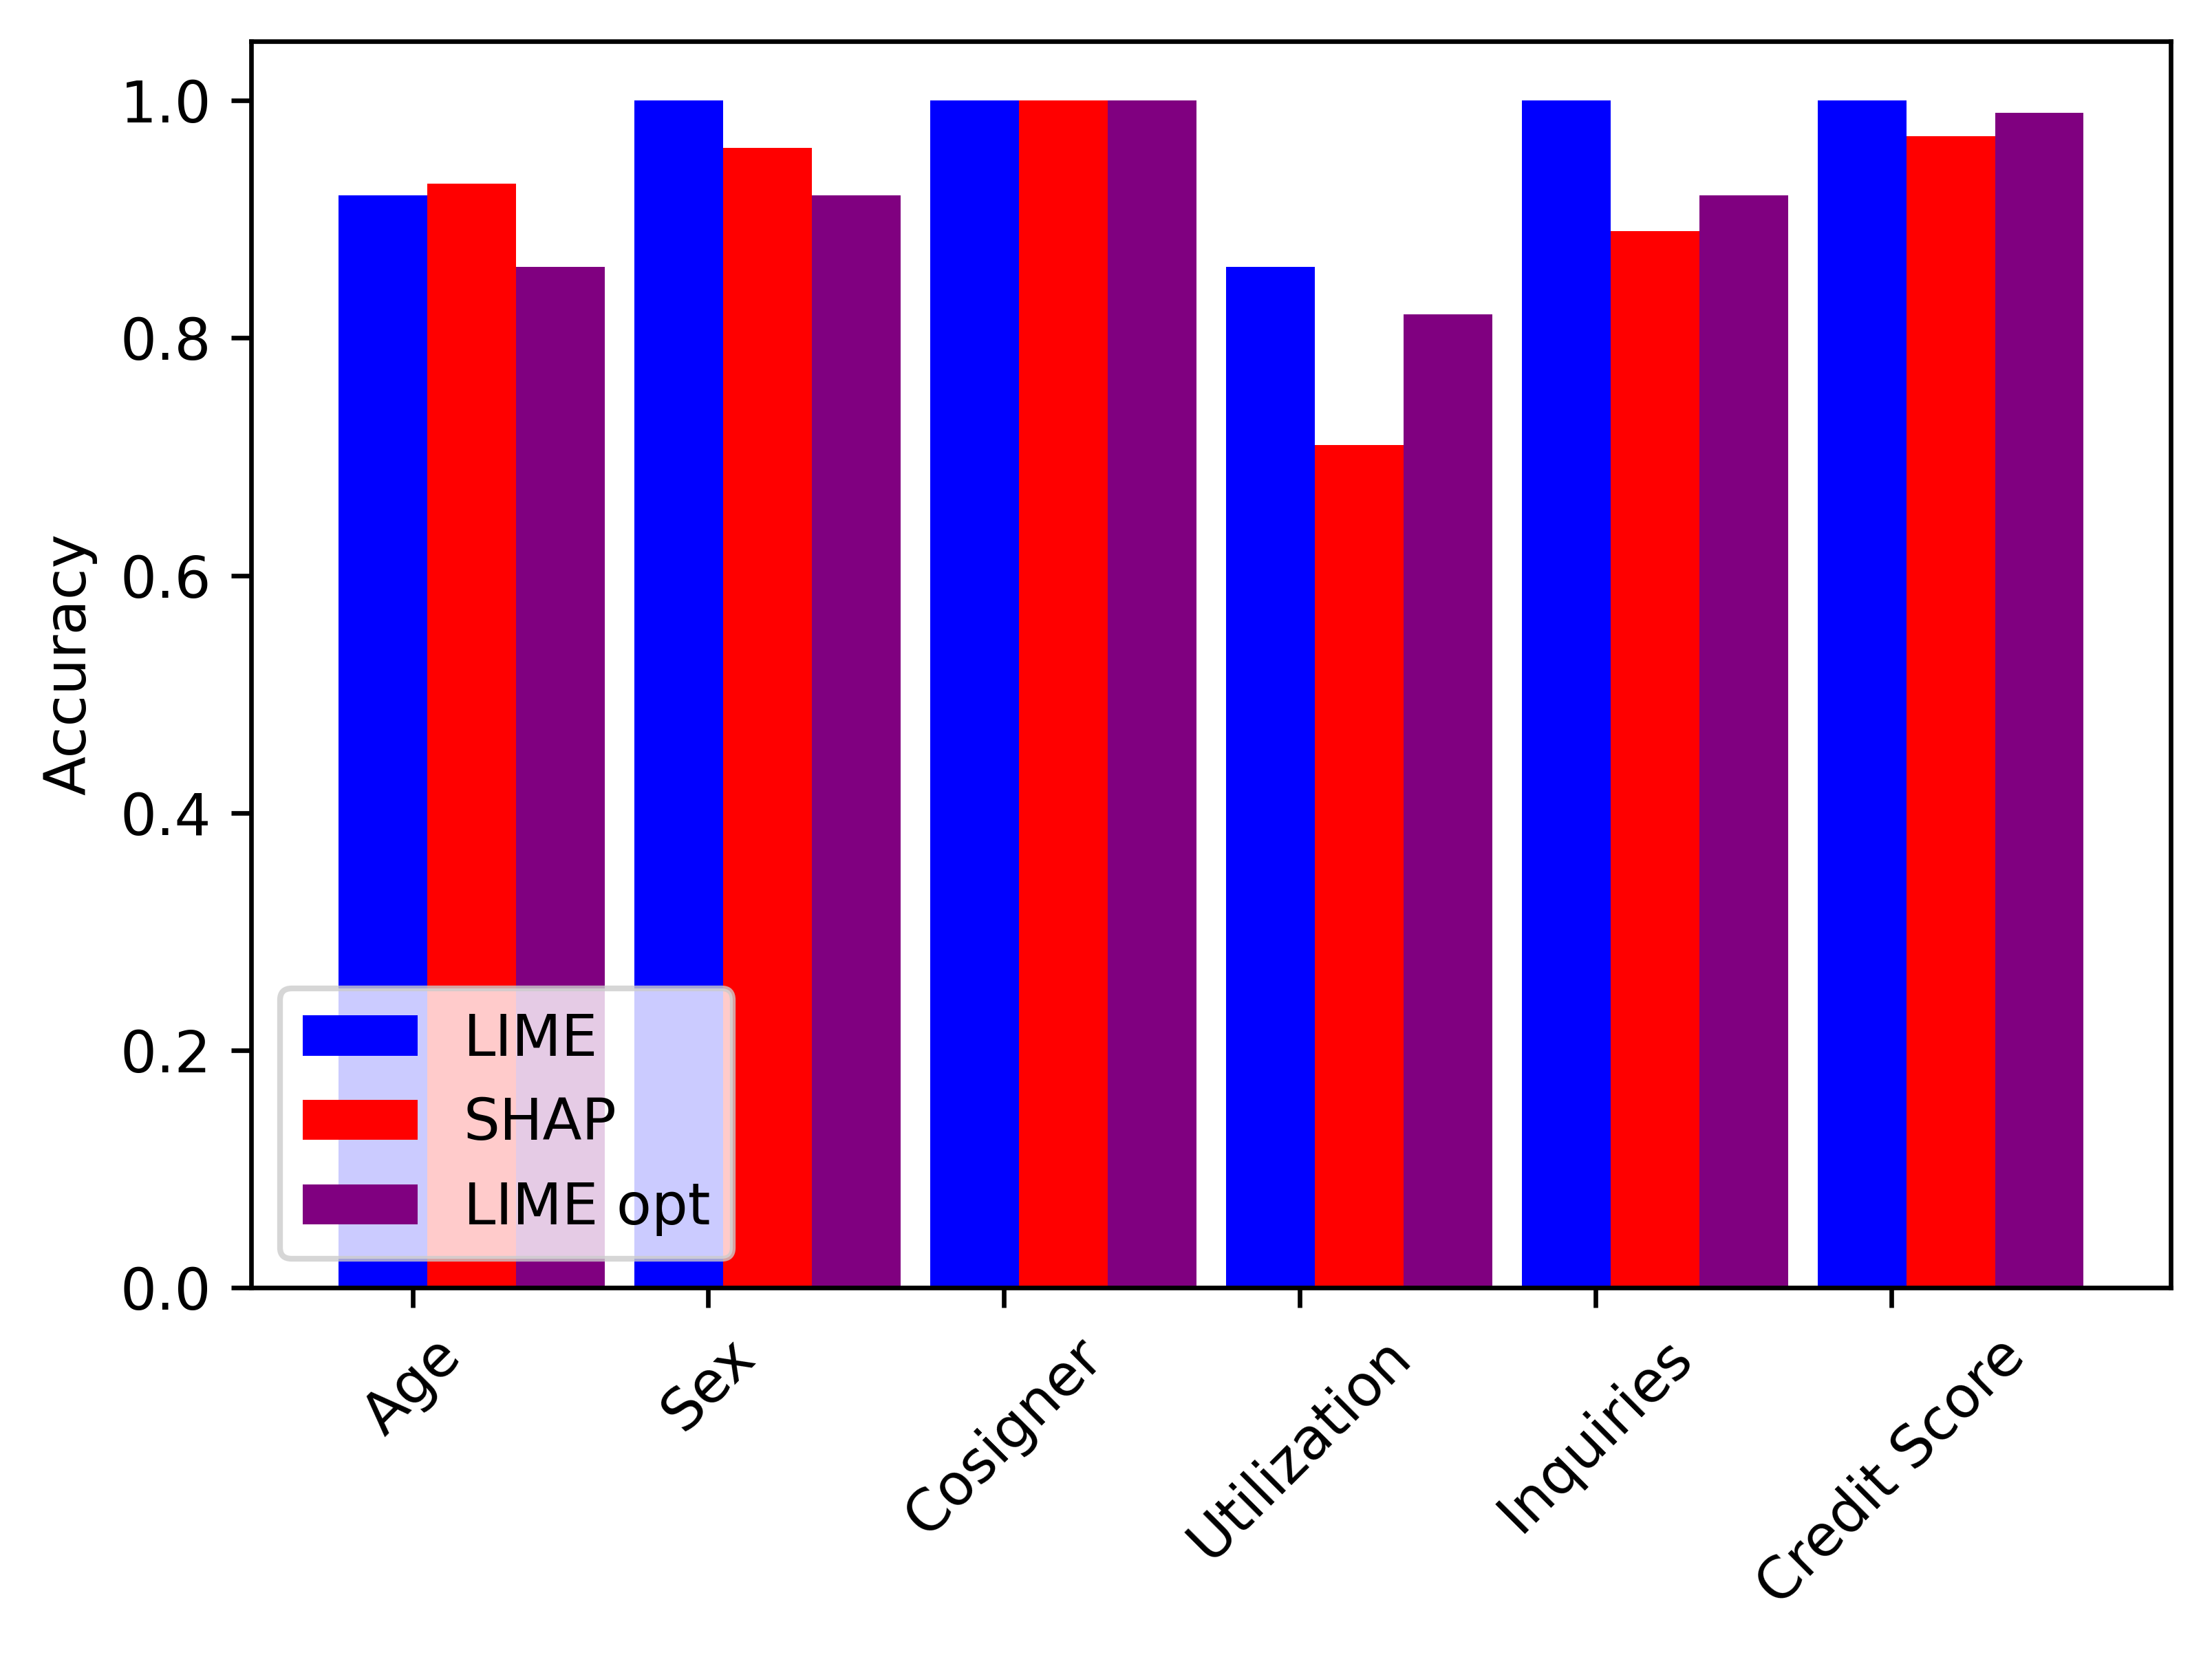
\includegraphics[width=\textwidth]{Figures/lime_shap_avg_acc.png}%{Figures/fig21.pdf}
                \caption{Sign Accuracy}
                \label{fig:lime_shap_Spearman_together}
                \end{subfigure}%
                \hspace{1cm}
                \begin{subfigure}{.27\textwidth}
                \centering
                %\fbox{\includegraphics[width=\textwidth,trim=0 10 70 70 mm, clip=true]{Figures/fig21.pdf}}%{Final_Figures/fig20.png}
                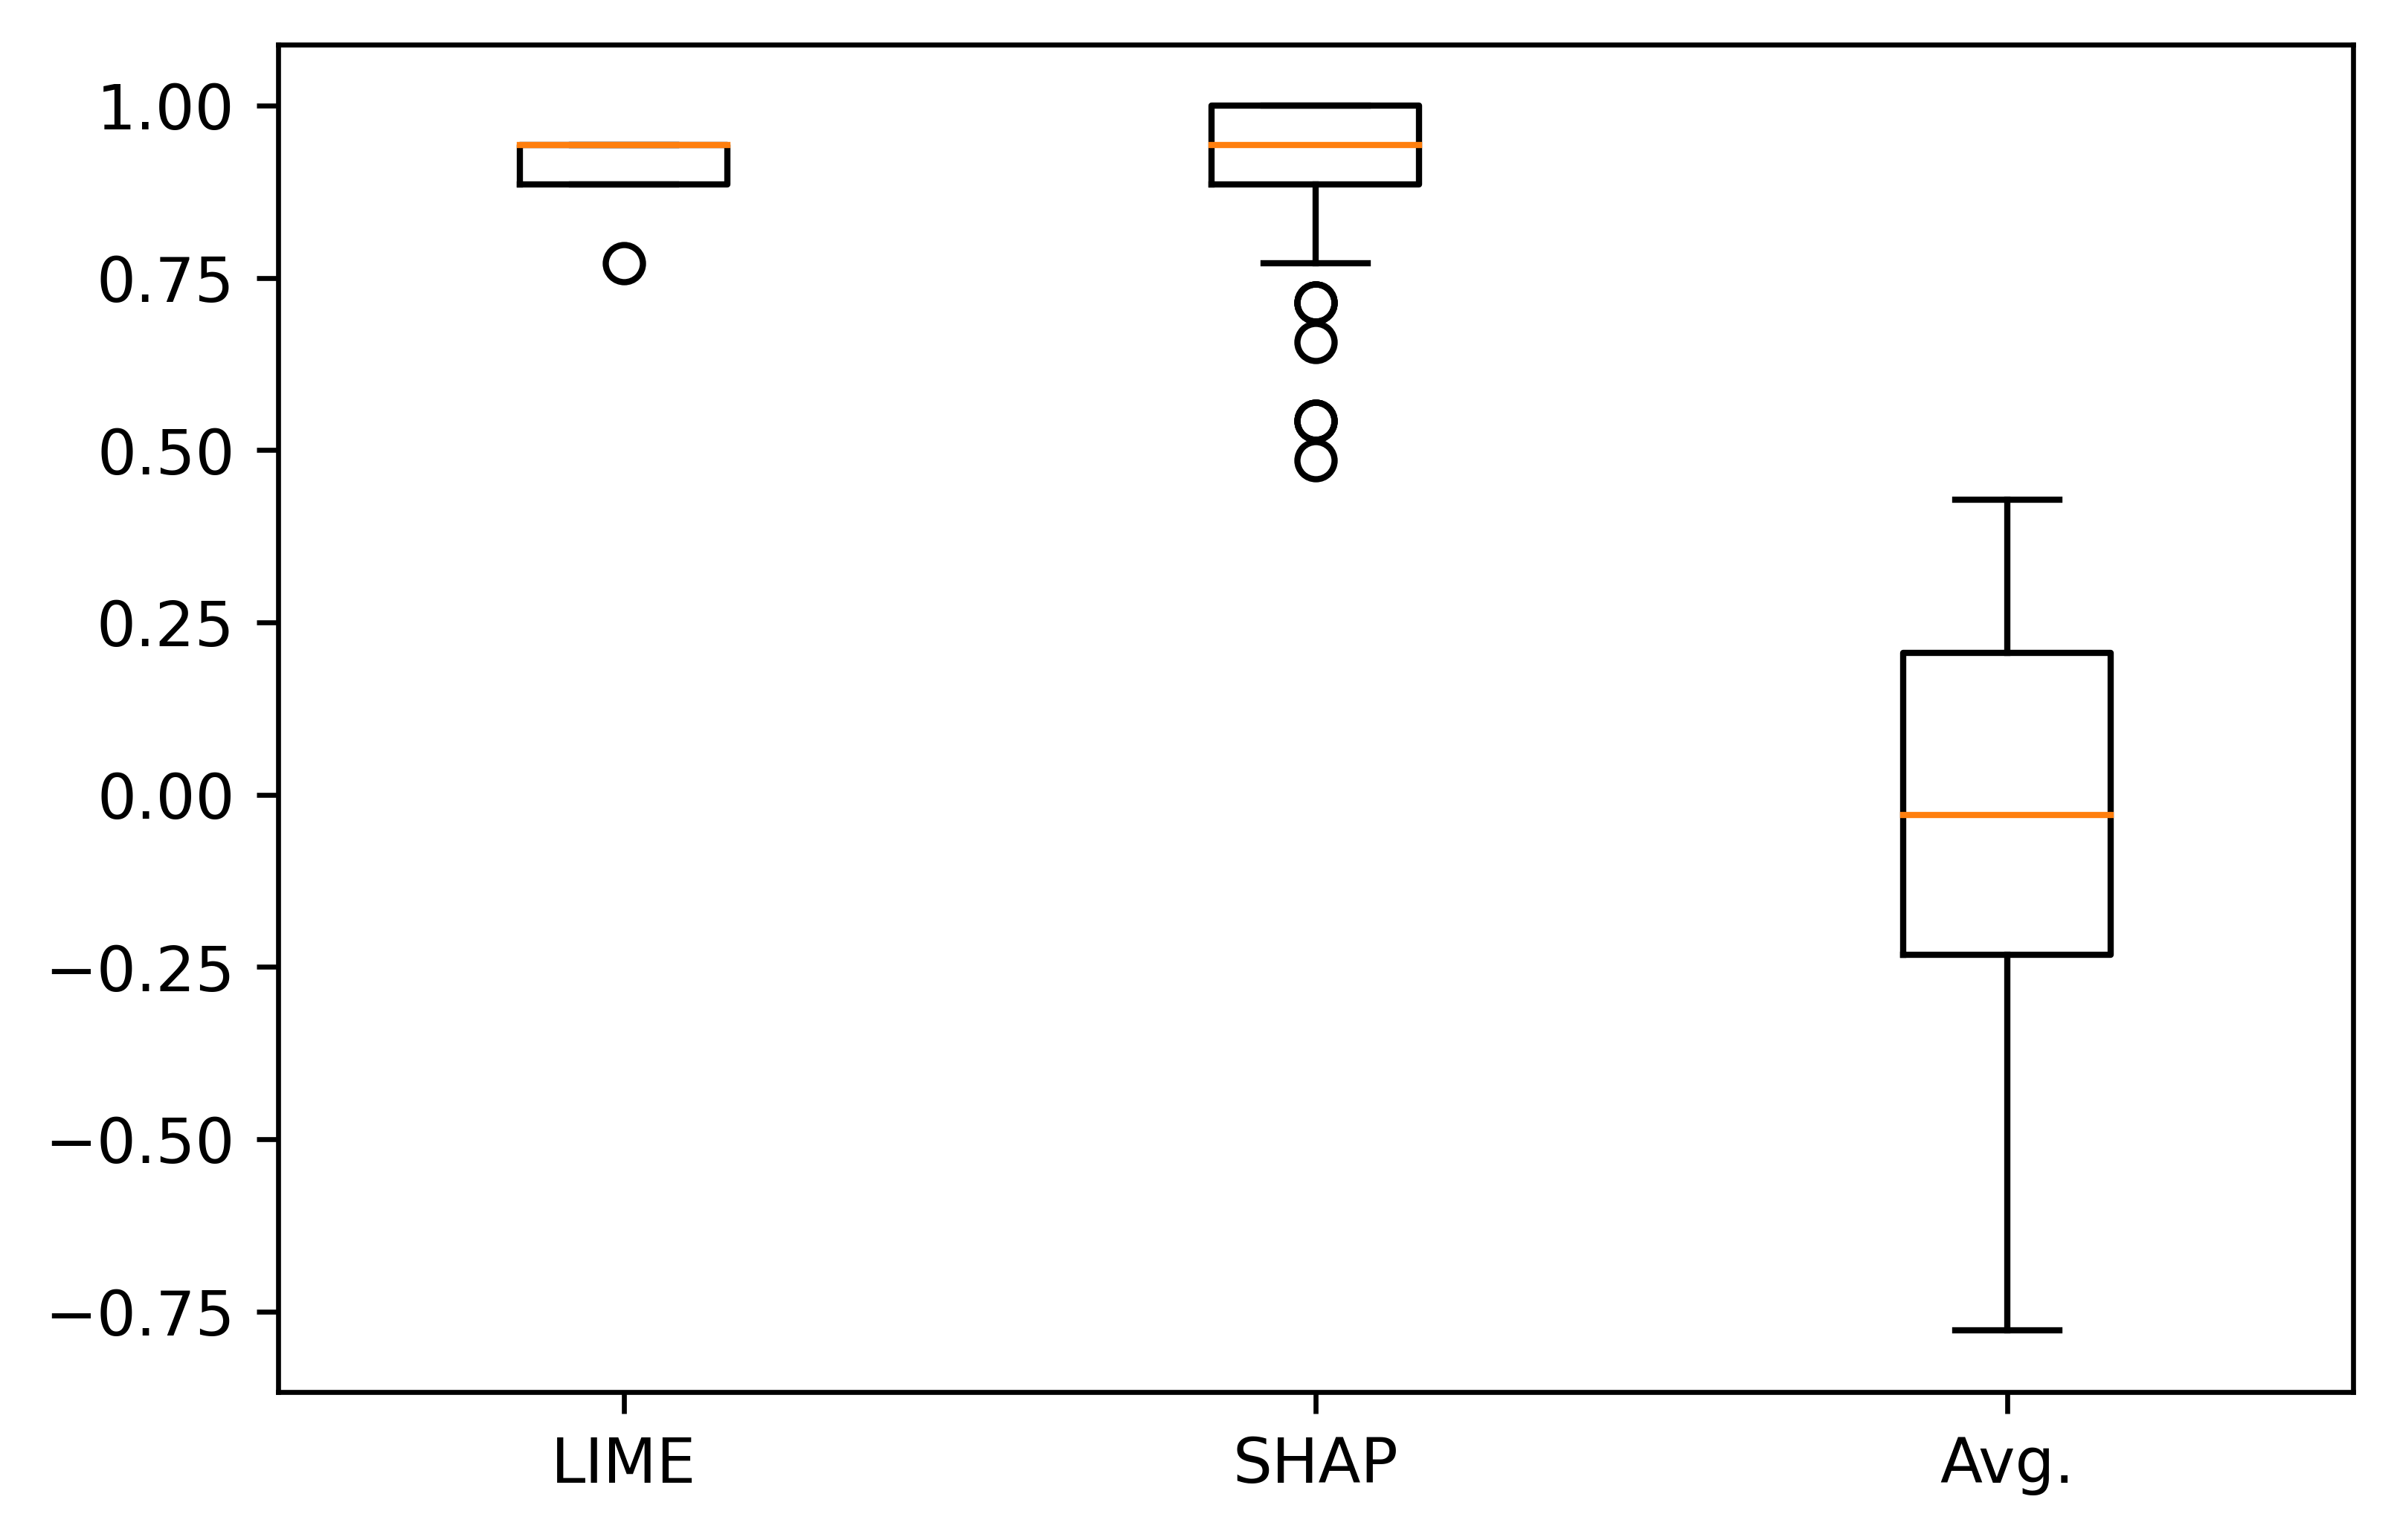
\includegraphics[width=\textwidth]{Figures/lime_shap_borda_spearmans.png}%{Figures/fig21.pdf}
                \caption{Importance Rankings}
                \label{fig:lime_shap_Spearman_together}
                \end{subfigure}%
                \begin{subfigure}{.27\textwidth}
                \centering
                %\fbox{\includegraphics[width=\textwidth,trim=0 10 70 70 mm, clip=true]{Figures/fig22.p}%{Final_Figures/fig21.png}
                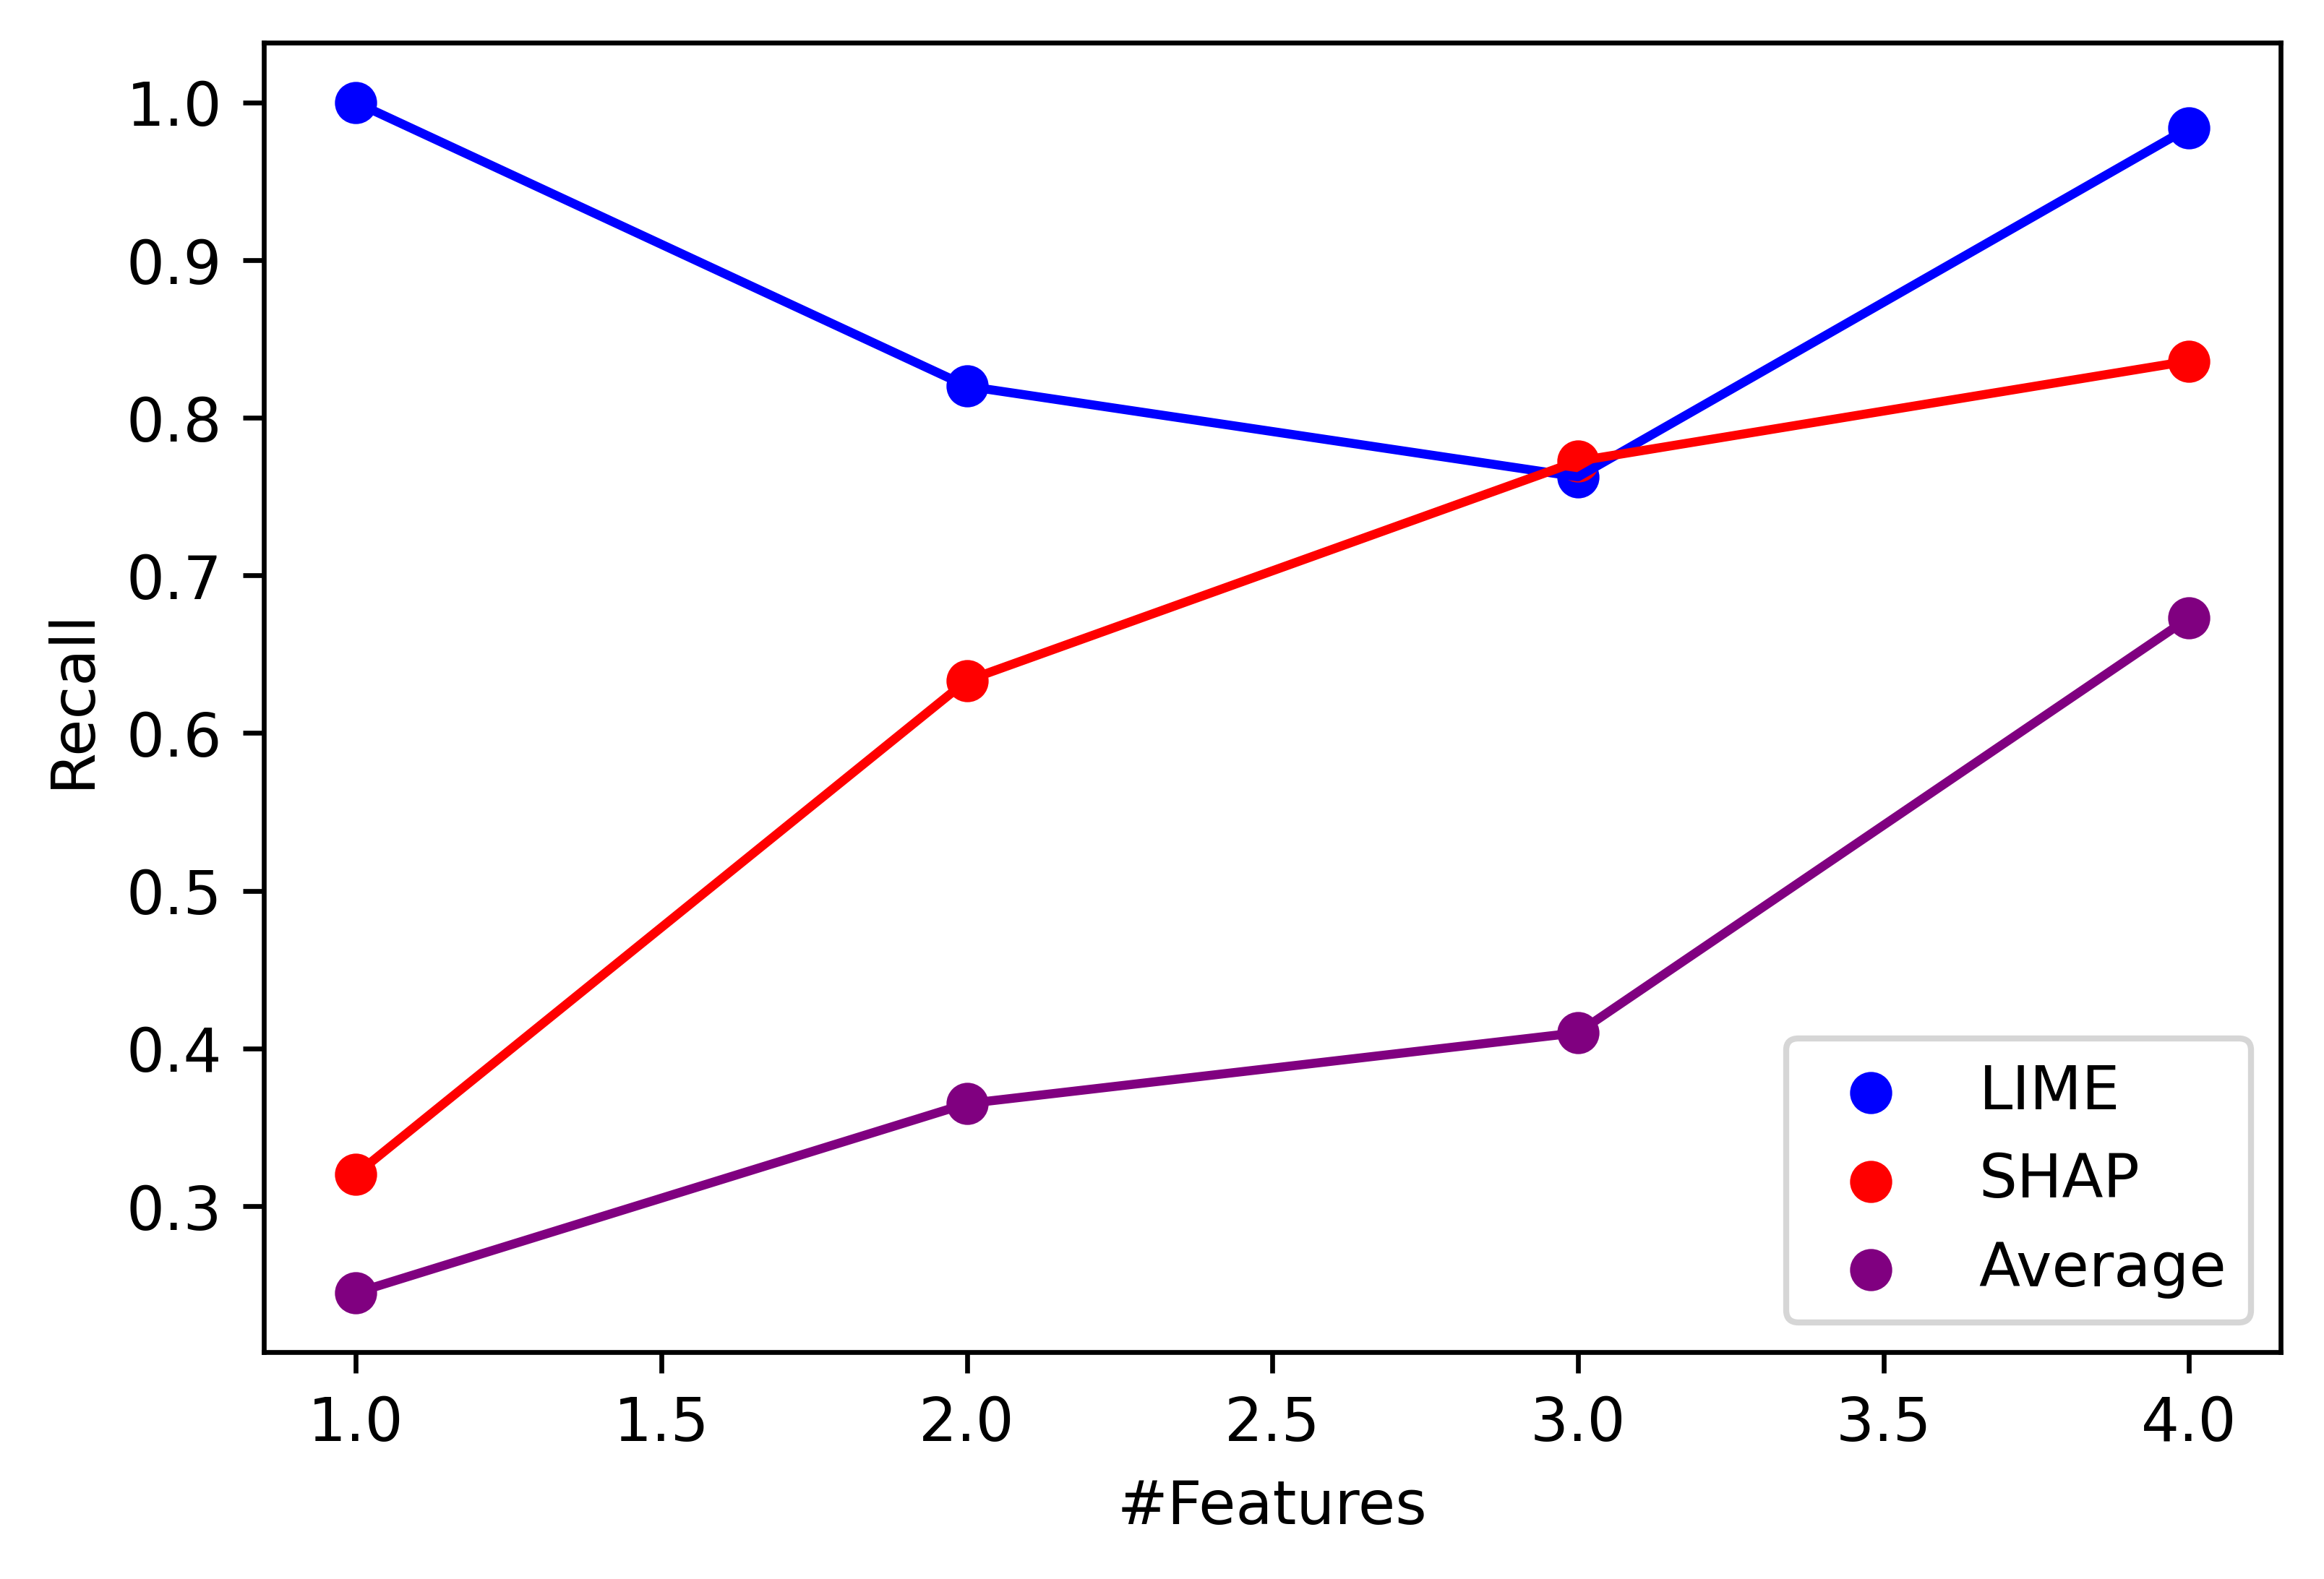
\includegraphics[width=\textwidth]{Figures/lime_shap_avg_recall.png}%{Figures/fig22.pdf}
                \caption{Recall}
                \label{fig:lime_shap_Spearman_together_recall}
                \end{subfigure}
            \caption{Violin plots showing the effect of averaging LIME and SHAP explanations together on explanation quality and the ability to identify the most important features. }
            \label{fig:lime_shap_spearman_plots}
            \end{figure}


        \subsubsection{Voting Ensembles}
            Prior experiments handled ensembles of explanations by constructing the final ranking by ranking the features according to the average importance given to them over the component explanations. We hypothesize that this strategy could be improved by adding sophistication using voting strategies such as the borda count.  

        \subsubsection{Increasing LIME Local Fidelity}
            In Section \ref{sec:} we established an association between the quality of a LIME explainer $\mathcal{E}$'s explanation of $y=\mathcal{M}(\xi)$ and whether $\mathcal{E}(\xi) = y$. We will explore here whether the accuracy of $\mathcal{E}$ on data in $\text{B}_\nu(\xi)$, the neighborhood of data samples within $\nu$ of $\xi$. 

        \subsubsection{Weak Learner LIMEs}

        \subsubsection{Pearl's Backdoor Adjustment}
            \label{sec:backdoor_adjustment}

    
    % add closed form for SHAP
    \subsection{Section \ref{sec:theoretical_considerations} Proofs and Experiments}    
        \subsubsection{Proofs}
        \paragraph{Setting of Theorem 1}
            We consider explaining a linear function $f:\mathbb{R}^d \rightarrow \mathbb{R}$ such that $f(\mathbf{x}) = \beta^T \mathbf{x}$ at the point $\mathbf{\xi}\in \mathbb{R}^d$ (which itself was sampled from $\mathcal{N}(0, \mathds{1}_d)$) using a LIME explainer with the following properties. Suppose that LIME samples random vectors $\{\mathbf{x}^{(n)}\}_{n=1}^N$ with $\mathbf{x}^{(n)} \sim \mathcal{N}(\mathbf{\xi},\mathds{1}_D)$ for each $n$ and, given a bandwidth parameter $\nu > 0$, weights their distances to $\mathbf{\xi}$ using an exponential kernel $\pi(\xi,\mathbf{x}) = exp(-\norm{\mathbf{\xi} - \mathbf{x}}_2^2/2\nu^2)$. In the Python LIME implementation, if $\xi$ has feature means $\mu_1,\ldots,\mu_D$ and standard deviations $s_1,\ldots,s_D$, then the samples $\mathbf{x}^{(n)}$ are given by $\sigma_1(z_1 + \mu_1),\ldots,\sigma_D(z_D + \mu_D)$ where each $z_i\sim \mathcal{N}(0,\mathbf{I})$. Since we assumed that $\xi \sim \mathcal{N}(0,\mathbf{I})$, we may assume that each sample is distributed according to $\mathcal{N}(0,\mathbf{I})$ as well. Thus, we may take $\sigma = 1$ in all proofs. 
        
        We assume that LIME follows one of its default settings to solve a ridge regression problem with the following loss function.
        \begin{equation*}
            (\mathbf{y} - \mathbf{X}\mathbf{u})^T \mathbf{W}(\mathbf{y} - \mathbf{X}\mathbf{u}) + (\mathbf{u} - \mathbf{u}_0)^T \Delta(\mathbf{u} - \mathbf{u}_0)
        \end{equation*}
        In this loss function, $\mathbf{X}$ is a data matrix $\mathbf{X} \in \mathbb{R}^{N\times D}$ whose $n^{th}$ row is $\mathbf{x}^{(n)}$ and $\mathbf{W} \in \mathbb{R}^{N\times N}$ is a diagonal weight matrix for each of the $n=1,\ldots,N$ samples with $w_{nn} = \pi(\xi,\mathbf{x}^{(n)}) = \exp(-\norm{\xi - \mathbf{x}^{(n)}}_2^2/2\nu^2)$. The response vector $\mathbf{y}\in \mathbb{R}^N$ is defined pointwise by $y_n = \beta^T \mathbf{x}^{(n)}$. We set the penalty parameter $\Delta\in \mathbb{R}^{D\times D}$ to $\Delta = \lambda \mathds{I}_{D\times D}$ so that $\Delta$ represents the $L_2$ ridge penalty with hyperparameter $\lambda$. There is another hyperparameter $\mathbf{u}_0 \in \mathbb{R}^D$ which is the target that $\mathbf{u}$ is to be shrunken toward.  We will set $\mathbf{u}_0 = 0$.

        In the proof $n$, and occasionally $n'$, will be used to index the $N$ data samples. $i,j,k$ and occasionally $l$ will be used to index the $D$ features. Individual data samples in the data matrix $\mathbf{X}$ will be represented with superscript notation, e.g. $\mathbf{x}^{(n)}$. Individual features of a sample will be indexed with subscript notation, e.g. $x^{(n)}_j$. We need not refer to whole rows or columns of $\mathbf{W}$, so it will be indexed entry-wise with $w_{nn}$ for $n=1,\ldots, N$.
    
    
        \paragraph{proof of Theorem 1a}
            The closed form solution to a generalized ridge regression with $\lambda = 1$ and $\mathbf{u}_0 = 0$ is
            \begin{equation*}
                \mathbf{u} = (\mathbf{X}^T \mathbf{W} \mathbf{X} + \mathbf{I})^{-1}(\mathbf{X}^T\mathbf{W}\mathbf{y})% + \Delta \mathbf{u}_0)
            \end{equation*}
                Defining $\hat{\mathbf{\Sigma}}_N = \frac{1}{N}(\mathbf{X}^T \mathbf{W} \mathbf{X} +  \mathbf{I}) \in \mathbb{R}^{D\times D}$ and $\hat{\mathbf{\Gamma}}_N = \frac{1}{N}\mathbf{X}^T \mathbf{W}\mathbf{y}\in \mathbb{R}^{D \times 1}$, we have by the weak law of large numbers that $\hat{\mathbf{\Sigma}}_N$ and  $\hat{\mathbf{\Gamma}}_N$ converge to matrices $\mathbf{\Sigma}=\lim_{N\rightarrow \infty} \mathds{E}[\hat{\mathbf{\Sigma}}_N]$ and $\mathbf{\Gamma}:=\lim_{N\rightarrow \infty} \mathds{E}[\hat{\mathbf{\Gamma}}_N]$ respectively.
                The ridge solution is then denoted $\mathbf{u} := \mathbf{\Sigma}^{-1}\mathbf{\Gamma}$. 
                
                % should actually switch k with i here since i indexes over 1,...,n
                We begin with the computation of $\mathbf{\Sigma}$. We have
                \begin{gather*}
                    \mathbf{\Sigma} = \lim_{N\rightarrow \infty} \frac{1}{N}\mathds{E}[\mathbf{X}^T \mathbf{W} \mathbf{X} + \mathbf{I}] 
                    = \lim_{N\rightarrow \infty} \frac{1}{N}\mathds{E}[\mathbf{X}^T \mathbf{W} \mathbf{X}] + \frac{1}{N} \mathbf{I} \\
                    = \lim_{N\rightarrow \infty} \frac{1}{N}\mathds{E}[\mathbf{X}^T \mathbf{W} \mathbf{X}]
                \end{gather*}
                where expectations are taken over the Wishart distributed random matrices $\mathbf{X}$.
               %  $$           
                Note that $\mathbf{\Gamma} = \frac{1}{N}\mathds{E}[\mathbf{X}^T \mathbf{W} \mathbf{y}]=\frac{1}{N}\mathds{E}[\mathbf{X}^T \mathbf{W} \mathbf{X} \beta]=\frac{1}{N}\mathds{E}[\mathbf{X}^T \mathbf{W} \mathbf{X}] \beta$, so 
                \begin{gather*}
                    \mathbf{\Gamma} = \mathbf{\Sigma} \beta  
                \end{gather*}
        Therefore, we need not actually calculate the expectations or invert $\mathbf{\Sigma}$. It follows that
        \begin{gather*}
            \mathbf{u} = \mathbf{\Sigma}^{-1} \mathbf{\Gamma} \beta = \beta
        \end{gather*}
     
    
        \paragraph{Proof of Lemma 1}
            Let $\mathbf{z} \in \mathbb{R}^N$. First, note that $\mathbf{W}$ induces the norm $\norm{\mathbf{z}}_\mathbf{W} = \sqrt{\mathbf{z}^T \mathbf{W} \mathbf{z}} = \norm{\mathbf{W}^{1/2}\mathbf{z}}_2$. Thus, $\mathbf{X}^T \mathbf{W} \mathbf{X}$ is positive semi-definite. 
            \begin{gather*}
                \mathbf{z}^T \mathbf{X}^T \mathbf{W} \mathbf{X} \mathbf{z} = (\mathbf{X} \mathbf{z})^T \mathbf{W} (\mathbf{X} \mathbf{z}) \\
                = \norm{\mathbf{W}^{1/2} \mathbf{X}\mathbf{z}}_2 \geq 0
            \end{gather*}
            
        \paragraph{Proof of Proposition 1}
            Since the eigenvalues of $\mathbf{A} + \mathbf{I}$ are $\lambda + 1$ for $\lambda$ in the spectrum of $\mathbf{A}$, the eigenvalues of $(\mathbf{A} + \mathbf{I})^{-1}$ have the form $\frac{1}{\lambda + 1}$. By Lemma 1, $\mathbf{A}$ is a symmetric positive semidefinite matrix, and so its singular values coincide with its eigenvalues. $\mathbf{I}$ is positive definite, and the sum of a positive definite matrix and a positive semidefinite matrix is positive definite. Moreover, the inverse of a positive definite matrix is also positive definite.  It follows that the singular values of $(\mathbf{A} + \mathbf{I})^{-1}$ take the form $\frac{1}{\sigma_k(\mathbf{A}) + 1}$ where $\sigma_k(\mathbf{A})$ is the $k^{\text{th}}$ singular value of $\mathbf{A}$. We can now bound $\norm{(\mathbf{A} + \mathbf{I})^{-1}\mathbf{A}}$ in terms of the largest and smallest singular values of $\mathbf{A}$. 
    
            For lower bounds:
            \begin{gather*}
                \norm{(\mathbf{A} + \mathbf{I})^{-1}\mathbf{A}} \geq \sigma_{\min}{(\mathbf{A} + \mathbf{I})^{-1}} \norm{\mathbf{A}} 
                = \frac{\sigma_{\max}(\mathbf{A})}{1 + \sigma_{\max}(\mathbf{A})} %\geq \frac{1}{1 + \sigma_{\max}(\mathbf{A})}
            \end{gather*}
            For upper bounds:
            \begin{gather*}
                \norm{(\mathbf{A} + \mathbf{I})^{-1}\mathbf{A}} \leq \sigma_{\max}{(\mathbf{A} + \mathbf{I})^{-1}} \sigma_{\max}(\mathbf{A}) \\
                \leq \frac{\sigma_{\max}(\mathbf{A})}{\sigma_{\min}(\mathbf{A})+1} \\
                \leq \frac{\sigma_{\max}(\mathbf{A})}{\sigma_{\min}(\mathbf{A})+1}
                \leq \frac{\sigma_{\max}(\mathbf{A})}{\sigma_{\min}(\mathbf{A})} = \kappa(\mathbf{A})
            \end{gather*}
            where $\kappa(\mathbf{A})$ is the condition number of $\mathbf{A}$. 
    
        \paragraph{Proof of Corollary 1}
            As $\nu \rightarrow 0$, $\mathbf{W} \rightarrow \mathbf{0}$, in which case $\mathbf{A}$ converges to $\mathbf{0}$ almost surely and the above bounds have a squeezing effect:
            \begin{equation*}
                0 \leq \norm{(\mathbf{A} + \mathbf{I})^{-1}\mathbf{A}} \leq 0 \implies (\mathbf{A} + \mathbf{I})^{-1}\mathbf{A} = \mathbf{0}
            \end{equation*}
    
    
        \paragraph{Proof of Corollary 2}
            If $\nu \rightarrow \infty$, $\mathbf{W} \rightarrow \mathbf{I}$ and so $\mathbf{A} \rightarrow \mathbf{X}^T \mathbf{X}$ almost surely. Then we have 
            \begin{equation*}
                \frac{\sigma_{\max}(\mathbf{X}^T \mathbf{X})}{\sigma_{\max}(\mathbf{X}^T \mathbf{X})+1} \leq \norm{(\mathbf{A} + \mathbf{I})^{-1}\mathbf{A}} \leq  \kappa(\mathbf{X}^T \mathbf{X})%\frac{\sigma_{\max}(\mathbf{X}^T \mathbf{X})}{\sigma_{\min}(\mathbf{X}^T \mathbf{X})+1} 
            \end{equation*}
            $\mathbf{X}^T \mathbf{X}$ is a Wishart random matrix, so its singular values are on the order of $\sqrt{ND}$. Thus, for $\sqrt{ND} >> 1$, the lower bound is approximately 1 and the upper bound  $\kappa(\mathbf{X}^T \mathbf{X})$ is at most 1 with high probability.  
            %https://arxiv.org/pdf/0810.0800.pdf
            % https://citeseerx.ist.psu.edu/document?repid=rep1&type=pdf&doi=ea7d6ef0f0c530ba591e0833935c4e17fa0794a6 thm3.2
            This can be shown using the following concentration inequality of \citep{edelman2005tails}.
            \begin{equation*}
                \mathds{P}[\kappa(\mathbf{X}^T \mathbf{X}) > 1] \leq c_1 c_2 \leq c_1 (\sqrt{D} + \sqrt{D-1})%\frac{1}{\sqrt{2\pi}} \left(\frac{6}{\mid N - D\mid + 1} \right)^{\mid N-D\mid + 1}
            \end{equation*}
    %https://arxiv.org/pdf/2106.07433.pdf#:~:text=In%20random%20matrix%20theory%2C%20the%20Gordon%E2%80%99s%20theorem%20says,be%20upper%20bounded%20by%20p%20m%2B%20p%20n.
            where $c_1 = \frac{N}{p} \frac{c_{N,D}}{c_{N-1,D+1}}$, $p=\frac{1}{2}(D-N+1)$, $c_{N,D} = \frac{\pi^{3N(N-1)/2}}{2^{ND/2}} \frac{\Gamma(3/2)}{\Gamma_N(3/2)\Gamma_N(p)}$, $\Gamma_N(z) = \pi^{N(N-1)/4} \prod_{i=1}^N \Gamma(z + (i+1)/2)$ is the multivariate gamma function and $c_2$ is the expected value of the largest singular value of a $D-1\times D+1$ matrix of i.i.d. standard Gaussians and the last inequality follows by Gordon's theorem \citep{vershynin2012introduction}.
    
            For fixed $D$, $c_{N,D} \in O\left(\frac{1}{\pi^{N^2} N^2 N!}\right)$. Thus, $c_1 \in O\left(\frac{1}{\pi^{N}N}\right)$. It follows that for sufficiently large $N$, $\mathds{P}[\kappa(\mathbf{X}^T \mathbf{X}) > 1]$ is sufficiently small so that $(\mathbf{A} + \mathbf{I})^{-1}\mathbf{A}$ is squeezed to a value near 1. %CHECK!
    
            
        \paragraph{proof of Theorem 2.}
            This follows immediately from \citep{StrumbeljErik2014Epma} and the assumption that each feature has zero mean.
    
        \subsubsection{Insights From Theoretical Results}
            \begin{itemize}
                \item Although explanations using discretized features may be more easily interpretable, they make the explanations less faithful
                \item Users should generally opt to set $N$ to be large 
                \item Users should generally set $\nu$ to be large, otherwise the LIME coefficients may be become zero
                %\item LIME becomes more unfaithful as the number of features $D$ grows. 
                \item The ridge penalty matters only when $\lambda \in O(N)$
            \end{itemize}
    
            \subsubsection{Simulation Experiments}
                \label{sec:simulation_experiments}
                For our simulation, we use LIME with and without discretization to explain a linear regressor $f(x) = .05 + .05x_1+ .2x_2+ .8x_3 -.5x_4 +x_5$ with $x_i \sim \mathcal{N}(0,1)$ for all $i$. $\nu$ is set to the default value. We pick 100 test set instances and explain each two sets of 100 LIME explainers. The first set of LIME explainers do not use feature discretization while the second set does. The $n^{th}$ explainer has its random seed set to $n$ in both sets. For each set of explainers, we plot the ratios $C_i:= e(x_j)_i/\beta_i$ for $i=1,\ldots,5$ in Figure \ref{fig:c_demo}.
    
                As we claimed in Section 3, the LIME explainers with no feature discretization generally have $C_i$ closer to $1$ than the LIME explainers with discretization. The difference is especially stark with $C_{1}$, which is always 1 with no discretization and between -10 and 20 with discretization. Note that when $C_i$ is negative, LIME has misidenified how feature $i$ impacts the output of $f$. Moreover, in accordance with Theorem 1 and \citep{garreau20theoretical}, we see that $C_i$ can differ significantly across $i$, indicating that $e(x_j)$ is not directly proportional to $\beta$ regardless of whether discretization is used. 
    
                \paragraph{Role of $\nu$ and $N$ on convergence}
    
                \begin{figure}[ht!]
                \centering
                    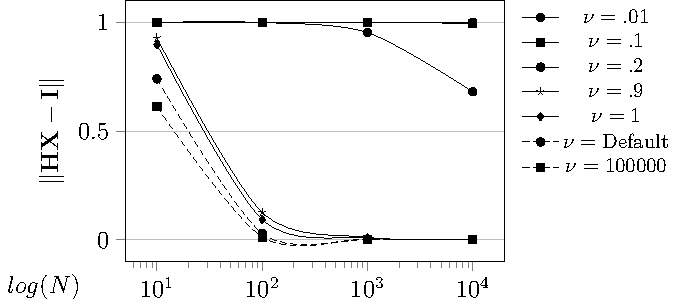
\includegraphics[height=.2\textwidth]{AppendixFigures/apx_lime_conv_nu_N.pdf}%{Figures/fig21.pdf}
                    \caption{Role of $\nu,N$ on $\norm{(\mathbf{X}^T \mathbf{W} \mathbf{X} + \mathbf{I})^{-1}\mathbf{X}^T\mathbf{W}\mathbf{X} - \mathbf{I}}$, with $D=4$}
                    \label{fig:nu_N_convergence}
                \end{figure}

                \paragraph{Role of $D$ on convergence}
    
                \begin{figure}[ht!]
                \centering
                    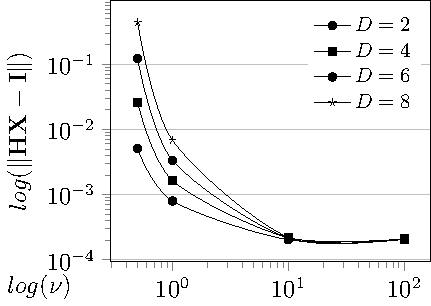
\includegraphics[width=.27\textwidth]{AppendixFigures/apx_lime_conv_D.pdf}%{Figures/fig21.pdf}
                    \caption{Role of $D$ on $\norm{(\mathbf{X}^T \mathbf{W} \mathbf{X} + \mathbf{I})^{-1}\mathbf{X}^T\mathbf{W}\mathbf{X} - \mathbf{I}}$ with $N=50000$}
                    \label{fig:nu_N_convergence}
                \end{figure}
    
                \paragraph{Upper Bounds on $\norm{ (\mathbf{X}^T \mathbf{W} \mathbf{X} + \mathbf{I})^{-1}\mathbf{X}^T\mathbf{W}\mathbf{X}}_2$}
                \begin{figure}[ht!]
                \centering
                    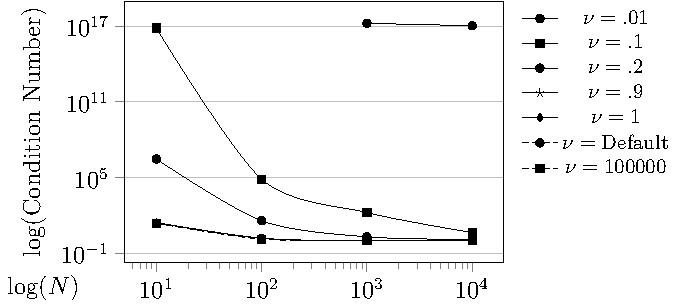
\includegraphics[height=.2\textwidth]{AppendixFigures/apx_lime_conv_cond.pdf}%{Figures/fig21.pdf}
                    \caption{Role of $\nu,N$ on upper bound of $\norm{(\mathbf{X}^T \mathbf{W} \mathbf{X} + \mathbf{I})^{-1}\mathbf{X}^T\mathbf{W}\mathbf{X}}$}
                    \label{fig:nu_N_convergence}
                \end{figure}
    
                \paragraph{Role of Discretization}
                %use fbox to tailor crop
                \begin{figure}[ht!]
                \centering
                    \begin{subfigure}{.27\textwidth}
                    \centering
                    %\fbox{\includegraphics[width=\textwidth,trim=0 10 70 70 mm, clip=true]{Figures/fig21.pdf}}%{Final_Figures/fig20.png}
                    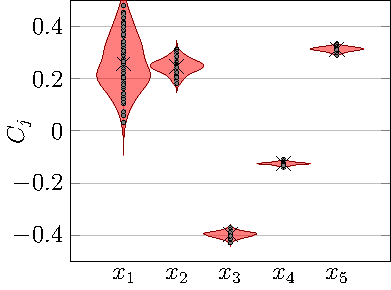
\includegraphics[width=\textwidth]{AppendixFigures/apx_lime_proportionality.pdf}%{Figures/fig21.pdf}
                    \caption{No discretization}
                    \label{fig:empirical_c}
                    \end{subfigure}%
                    \hspace{3cm}
                    \begin{subfigure}{.27\textwidth}
                    \centering
                    %\fbox{\includegraphics[width=\textwidth,trim=0 10 70 70 mm, clip=true]{Figures/fig21.pdf}}%{Final_Figures/fig20.png}
                    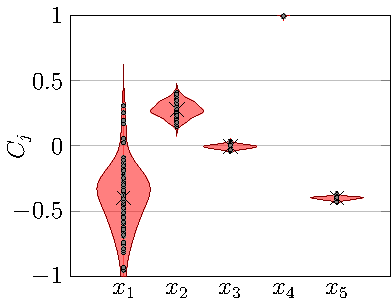
\includegraphics[width=\textwidth]{AppendixFigures/apx_lime_disc_proportionality.pdf}%{Figures/fig21.pdf}
                    \caption{Discretization allowed}
                    \label{fig:theoretical_cs}
                    \end{subfigure}%
                \caption{Empirical $C_i$ for 100 applicants from 100 LIMEs with/without discretization, and all other parameters set to the defaults}
                \label{fig:c_demo}
                \end{figure}
    

    


    \subsection{Details on Econometric Case Study}
        Feature interpretations were obtained from \citep{HunterWilliamC1996Tcah}.
        \begin{table}[]
            \centering
            \begin{tabular}{|l|l|l|}
            \hline
            \textbf{Feature} & \textbf{Meaning}                   & \textbf{Range}                \\ \hline
            %gdlin            & credit history meets guidelines    & binary                        \\ \hline
            good credit            & credit history meets guidelines    & binary                        \\ \hline
            %typur            & type of purchaser of loan          & 0,1,2,\textbackslash{}ldots,9 \\ \hline
            purchaser type            & type of purchaser of loan          & 0,1,2,\textbackslash{}ldots,9 \\ \hline
            %inson            & \makecell{approved for private mortage insurance (PMI)}                      & binary                        \\ \hline
            PMI approved            & \makecell{approved for private mortage insurance (PMI)}                      & binary                        \\ \hline
            %prop             & type of property                   & binary                        \\ \hline
            multi family     & \makecell{purchasing 2-4 family home \\ versus 1 family home or condo } \\ \hline
            unver            & unverifiable info                  & binary                        \\ \hline
            %fixadj           & fixed or adjustable rate           & binary                        \\ \hline
            fixed rate           & fixed or adjustable rate           & binary                        \\ \hline
            %pubrec           & filed bankruptcy                   & binary                        \\ \hline
            bankruptcy           & filed bankruptcy                   & binary                        \\ \hline
            %vr               & tract vac rte \textgreater msa med & binary                        \\ \hline
            value rate               & \makecell{whether the rental income in tract \\ divided by estimate of value \\\ of rental property \textgreater Boston median} & binary                        \\ \hline
            %obrat            & \makecell{percentages of housing expenditures \\ and other obligations \\ normalized by total income}    & {[}0,100{]}                   \\ \hline
            debt rate           & \makecell{percentages of housing expenditures \\ and other obligations \\ normalized by total income}    & {[}0,100{]}                   \\ \hline
            old              & applicant age \textgreater Boston median & binary                        \\ \hline
            married          & if applicant married               & binary                        \\ \hline
            gift             & gift as down payment               & binary                         \\
            \end{tabular}
            \caption{Feature meanings and ranges for the case study}
            \label{tab:case_study_features}
        \end{table}

\subsection{Guidance For Use of Post-Hoc Explainers}
    \subsubsection{Compare Explanations With Those From Decision Trees}

    \subsubsection{Causal Graph}


\section{Nonlinear Experiments}




\end{document}
%%%%%%%%%%%%%%%%%

